\documentclass[fleqn,twocolumn,11pt]{wlscirep}
\usepackage[utf8]{inputenc}
\usepackage[T1]{fontenc}
\usepackage{bm}
\usepackage{color}
\linespread{1.0}
\newcommand{\onlinecite}[1]{\hspace{-1 ex} \nocite{#1}\citenum{#1}}
\usepackage{color}
\usepackage{alltt,dsfont}
\usepackage{appendix}
\usepackage{amsmath,amssymb}
\usepackage{braket}
\usepackage[capitalise]{cleveref}
\usepackage{ulem}
\usepackage{float}
\usepackage{graphicx,subfigure,amsmath,bbm}

\usepackage{lipsum}
\usepackage{nameref}
% folowing  must be in this order
\usepackage{hyperref}
\usepackage{cleveref}
\renewcommand{\familydefault}{\sfdefault}
\usepackage[]{sfmath}     %Equations in Arial
\newcommand{\minus}{\scalebox{0.75}[1.0]{$-$}}
\usepackage[export]{adjustbox}
\usepackage{subscript}
\usepackage{titlesec,setspace}

\renewcommand{\figurename}{{\bf Fig}}


\begin{document}

\title{Orbital structure of the effective pairing interaction in the high-temperature superconducting cuprates}

\author[1]{Peizhi Mai}
\author[2]{Giovanni Balduzzi}
\author[3,4]{Steven Johnston}
\author[1,5,*]{Thomas A. Maier}
\affil[1]{Center for Nanophase Materials Sciences, Oak Ridge National Laboratory, Oak Ridge, TN 37831-6164, USA}
\affil[2]{Institute for Theoretical Physics, ETH Z{\"u}rich, 8093 Z{\"u}rich, Switzerland}
\affil[3]{Department of Physics and Astronomy, University of Tennessee, Knoxville, Tennessee 37996-1200, USA}
\affil[4]{Joint Institute for Advanced Materials at The University of Tennessee, Knoxville, TN 37996, USA}
\affil[5]{Computational Sciences and Engineering Division, Oak Ridge National Laboratory, Oak Ridge, TN, 37831-6494, USA}

\affil[*]{e-mail: maierta@ornl.gov }
\date{\today}

\begin{abstract}
The nature of the effective interaction responsible for pairing in the high-temperature superconducting cuprates remains unsettled. This question has been studied extensively using the simplified single-band Hubbard model, which does not explicitly consider the orbital degrees of freedom of the relevant CuO$_2$ planes. Here, we use a dynamical cluster quantum Monte Carlo approximation to study the orbital structure of the pairing interaction in the three-band Hubbard model, which treats the orbital degrees of freedom explicitly. We find that the interaction predominately acts between neighboring copper orbitals, but with significant additional weight appearing on the surrounding bonding molecular oxygen orbitals. By explicitly comparing these results to those from the simpler single-band Hubbard model, our study provides strong support for the single-band framework for describing superconductivity in the cuprates.
\end{abstract}

\maketitle


\section*{Introduction}
Cuprate superconductivity emerges in their quasi-two-dimensional (2D) CuO$_2$ planes after doping additional carriers into these layers. The undoped parent compounds are charge transfer insulators due to the large Coulomb repulsion $U_{dd}$ on the Cu 3$d$ orbitals, and, to a good approximation, a spin-$\tfrac{1}{2}$ hole is located on every Cu 3$d_{x^2-y^2}$ orbital. This situation is well described by a half-filled 2D square lattice Hubbard model or Heisenberg model in the large $U_{dd}$ limit. 

Upon doping, the additional holes or electrons primarily occupy the O or Cu orbitals, respectively. The minimal model capturing this asymmetry is the three-band Hubbard model, which explicitly accounts for the Cu $3d_{x^2-y^2}$, O $2p_{x}$, and $2p_y$ orbitals (Fig.~\ref{Fig:PairStructure}{\bf  a})~\cite{EmeryPRL1987}. Even at finite doping, the low energy sector of the three-band model can be mapped approximately onto an effective single-band Hubbard model~\cite{ZhangRice}. One expects this in the case of electron-doping since the additional carriers go directly onto the Cu sublattice, on which the holes of the undoped materials already reside. The case of hole-doping, however, is more subtle. Here, the additional carriers predominantly occupy the O sublattice due to the large $U_{dd}$ on the Cu orbital, and the appropriateness of a single-band model is less clear. In their seminal work, Zhang and Rice ~\cite{ZhangRice} argued that the doped hole effectively forms a spin-singlet state with a Cu hole, the ``Zhang-Rice singlet'' (ZRS, Fig.~\ref{Fig:PairStructure}{\bf b}), which then plays the same role as a fully occupied or empty site in an effective single-band model, again facilitating a single-band description.

The nature of the single-band 2D Hubbard model's pairing interaction has been extensively studied \cite{Maier4PRL, Maier07, Maier08, Kyung09, Gull14, Maier16}. Detailed calculations of its momentum and frequency structure using dynamical cluster approximation (DCA) quantum Monte Carlo (QMC) \cite{Maier4PRL} find that it is well described by a spin-fluctuation exchange interaction \cite{Maier07}. The single-band model, however, cannot provide any information on the orbital structure of the interaction. For example, in the hole doped case, the spins giving rise to the spin-fluctuation interaction are located on the Cu sublattice, while the paired holes are moving on the O $p_{x/y}$ sublattice. This situation can produce a different physical picture than if the interaction and the pairs both originate from the same orbital on the same lattice \cite{Lau11,Ebra14,Ebra16,Adolphs16,Jiang20}. And indeed, studies have observed two-particle behavior in a two sublattice system that is not observed in a one-lattice system \cite{Moeller12}. Moreover, an analysis of resonant inelastic x-ray scattering studies has found that a single-band model fails to describe the high-energy magnetic excitations near optimal doping \cite{Chen13}. For these reasons, numerous numerical studies of the three-band Hubbard model have been carried out to date \cite{Dopf, Arrigoni, Kung, Thomale, Weber1, Weber2, Weber3, Weber4, Acharya, Huang, Cui,Biborski,Zegrodnik}; however, the crucial task of studying its effective interaction, and, in particular, determining its orbital structure is currently lacking. Such a study will also provide new insight into the nature of high-temperature superconductivity that is not available from the previous single-band studies. In this letter, we use a QMC-DCA method to explicitly calculate the orbital and spatial structure of the effective interaction in a realistic three-band CuO$_2$ model, and compare the results with those obtained from a single-band model.

\section*{Results and Discussion}

\subsection*{Pairing structure of the three-band model}
To study the structure of the pairing interaction, we solved the Bethe-Salpeter equation (BSE) in the particle-particle singlet channel to obtain its leading eigenvalues and  eigenvectors~\cite{supplement, Maier4PRL} (see methods). 
Fig.~\ref{Fig:PairStructure}{\bf c} shows the leading eigenvalue of the BSE for the three-band model as a function of hole concentration $n_h$ obtained on a $4\times 4$ cluster with $\beta=1/k_\mathrm{B}T=16$~eV$^{-1}$. We find that it always corresponds to a $d$-wave superconducting state~\cite{KirtleyReview} and is larger for hole-doping ($n_h>1$) compared to electron-doping ($n_h<1$). The latter observation suggests a particle-hole asymmetry in $T_\mathrm{c}$ consistent with experiments and prior studies of the single and two-band Hubbard models~\cite{Maier3,Macridin}. (Although $\lambda_d$ is largest at half-filling, we expect that it asymptotically approaches one as the temperature decreases but never actually cross one due to the opening of a Mott gap. We observe such behavior in explicit calculations on smaller three-band clusters, see Fig. S1~\cite{supplement}.)

\begin{figure}[hbt!]
\centering
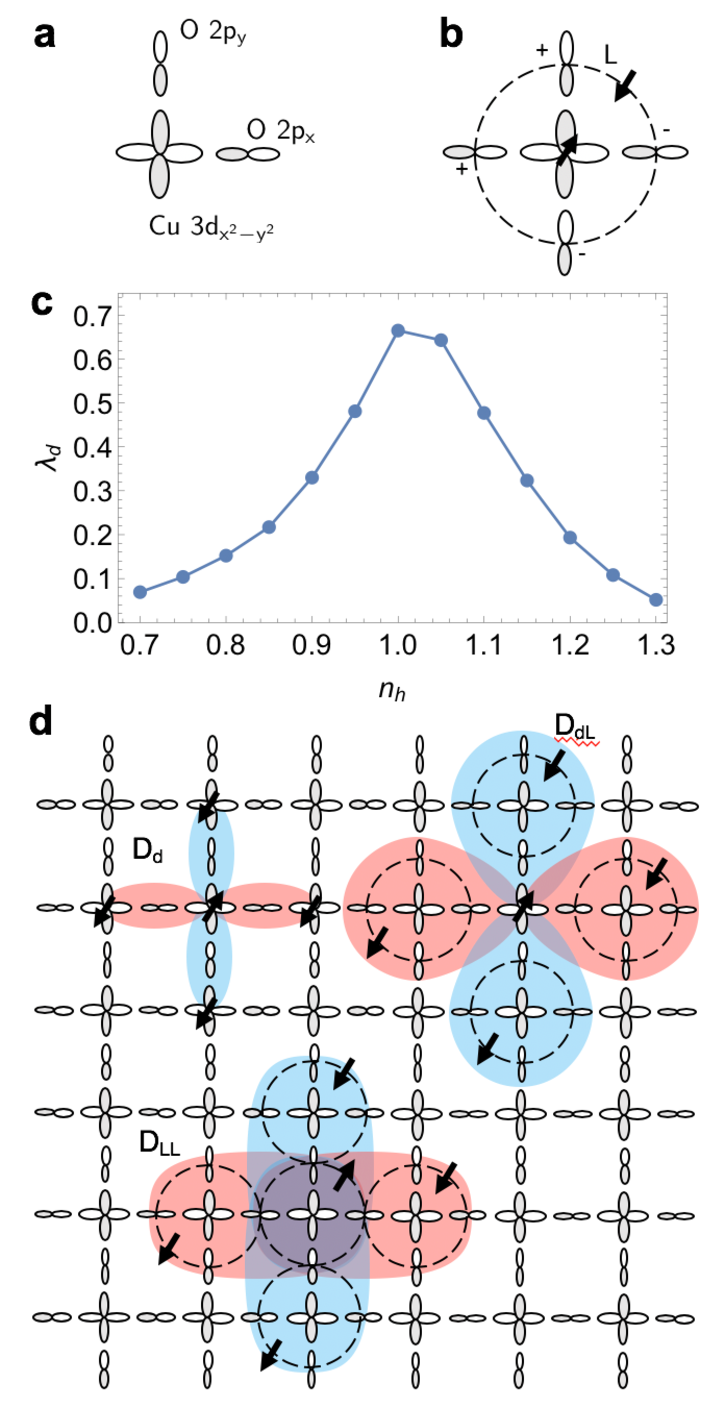
\includegraphics[width=\linewidth]{./Figures/Figure1.pdf}
\caption{{\bf A cartoon sketch of the three-band basis and the orbitals relevant to the Zhang-Rice Singlet.} {\bf a} The orbital basis of the three-band Hubbard model. {\bf b} Sketch of the bonding ligand ($L$) molecular orbital surrounding a central Cu-$d$ orbital. {\bf c} Leading BSE eigenvalue $\lambda_d$ vs $n_h$ for a $4\times4$ cluster at $\beta=16$ ~eV$^{-1}$. {\bf d} Sketches of some ways a pair can form with a $d$-wave symmetry.  Here, $D_{d}$ and $D_{dL}$ pair a Cu $3d$ hole with a hole on the neighboring Cu-$d$ and $L$ molecular orbital, respectively, while $D_{LL}$ pairs holes on neighboring O-$L$ orbitals.}
\label{Fig:PairStructure}
\end{figure}

\begin{figure*}[ht]
\centering
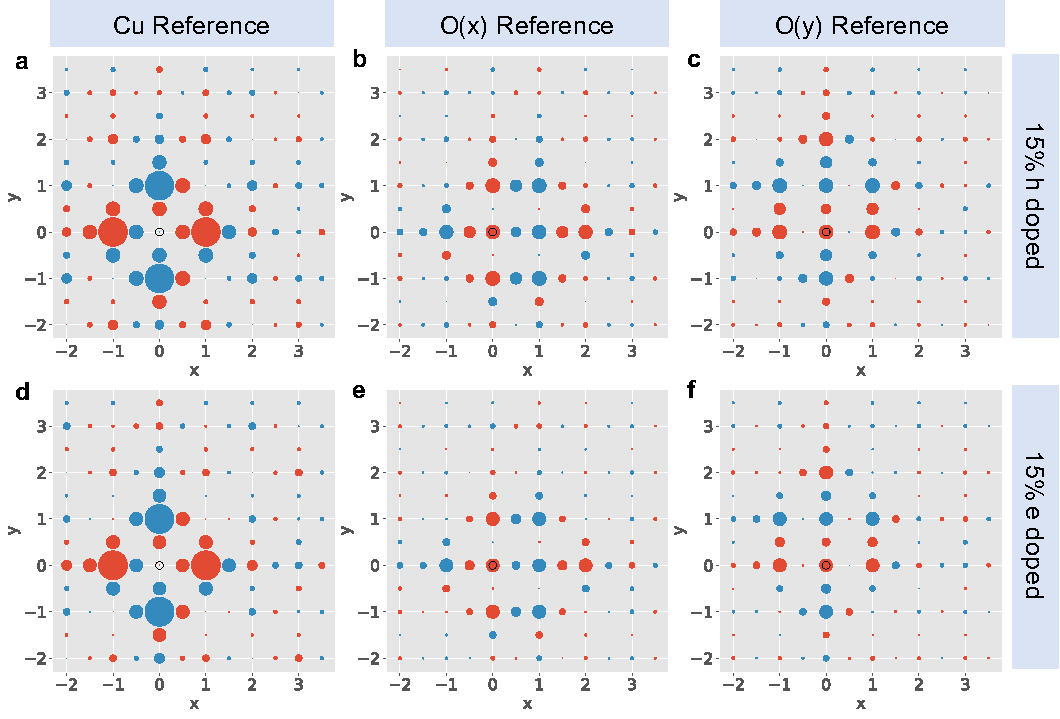
\includegraphics[width=\linewidth]{./Figures/Figure2.pdf}
\caption{{\bf Pairing structure of the three-band model.} The real space components of the leading  particle-particle BSE  (symmetrized) eigenvector for the three-band model at optimal doping and $\beta=10$ ~eV$^{-1}$ on a $6\times6$ cluster. Each column describes the pairing between a Cu $d$ (or O $p_x$, $p_y$) reference site and all other orbitals as a function of distance. All panels set the Cu-$d$ orbital at the origin, as labelled.}
\label{Fig:DCAPairStructure}
\end{figure*}

We now analyze the spatial and orbital structure of the leading eigenvector $\phi_{\alpha\beta}({\bf k})$ ($\alpha$ and $\beta$ denote orbitals), 
by Fourier transforming $\phi_{\alpha\beta}({\bf k})$ to real space to obtain $\phi_{{\bf r}_\beta}({\bf r}_{\alpha})$, where ${\bf r}_\beta$ denotes the position of the orbital taken as the reference site. We employed a $6\times6$ cluster to allow for long-ranged pairing correlations at $T=0.1$~eV. While this relatively high temperature is needed to mitigate the Fermion sign problem, we have found that the leading eigenvector changes very slowly as the system cools (see Supplementary Fig. 2)~\cite{supplement}. 
For example, we can reach much lower temperatures on $2\times2$ clusters, where we resolve the 
superconducting $T_c$ explicitly (see Supplementary Fig. 1)~\cite{supplement}. In that case, we observe that while the eigenvalue has a strong temperature dependence near $T_c$, its corresponding eigenvector does not vary much with temperature. From here on, we focus on results obtained at optimal (15\%) hole- or electron-doping. We have obtained similar results for different cluster sizes and for finite $U_{pp}$ (see Supplementary Figs. 3 and 4)~\cite{supplement}, indicating that our conclusions are robust across much of the model phase space. 


In the single-band Hubbard model, the pairs are largely comprised of carriers on nearest neighbor sites in a $d$-wave state, i.e. with a positive (negative) phase along the $x$- ($y$)-directions. The internal structure of the pairs in the three-band model seems more complicated~\cite{Moreo}. The real-space structure of $\phi_{{\bf r}_\beta}({\bf r}_\alpha)$ shown in Figs.\ref{Fig:DCAPairStructure} {\bf a}-{\bf c} and Figs.\ref{Fig:DCAPairStructure} {\bf d}-{\bf f} for the hole- and electron-doped cases, respectively, display an extended and rich orbital structure. Here, the size and color of the data points indicate the strength and phase of $\phi_{{\bf r}_\beta}({\bf r}_\alpha)$, respectively, on each site after adopting the central Cu $3d_{x^2-y^2}$ or O $2p_{x,y}$ orbital as a reference site at ${\bf r}_\beta$. The form factors $\phi_{{\bf r}_\beta}({\bf r}_\alpha)$ are similar for both electron and hole doping, decaying over a length scale of $\sim 2$--$3$ lattice constants. Moreover, while the $d$-wave pairing between nearest Cu sites dominates, there is also a significant contribution from $d$-$p$ pairing, with a comparable amplitude for up to the third-nearest (unit-cell) neighbors. The pairing between the individual O $2p_{x,y}$ orbitals is much weaker in comparison. 


\subsection*{Pairing in molecular basis}
We now transform the leading eigenvector for the hole-doped case from the O $p_x$ and $p_y$ basis to the bonding $L$ and anti-bonding $L^\prime$ basis (Fig.~\ref{Fig:PairStructure}d). These combinations, formed from the four O orbitals surrounding a Cu cation, are the relevant states for the ZRS, in which the doped holes are argued to reside in. The bonding $L$ state strongly hybridizes with the central Cu 3$d_{x^2-y^2}$ orbital (Fig.~\ref{Fig:PairStructure}{\bf  b}), while the anti-bonding $L^\prime$ state does not. The resulting antiferromagnetic exchange interaction between the Cu and $L$ holes is then argued to bind them into the Zhang-Rice spin-singlet state, which provides the basis for the mapping onto a single-band model.


\begin{figure*}[ht]
\centering
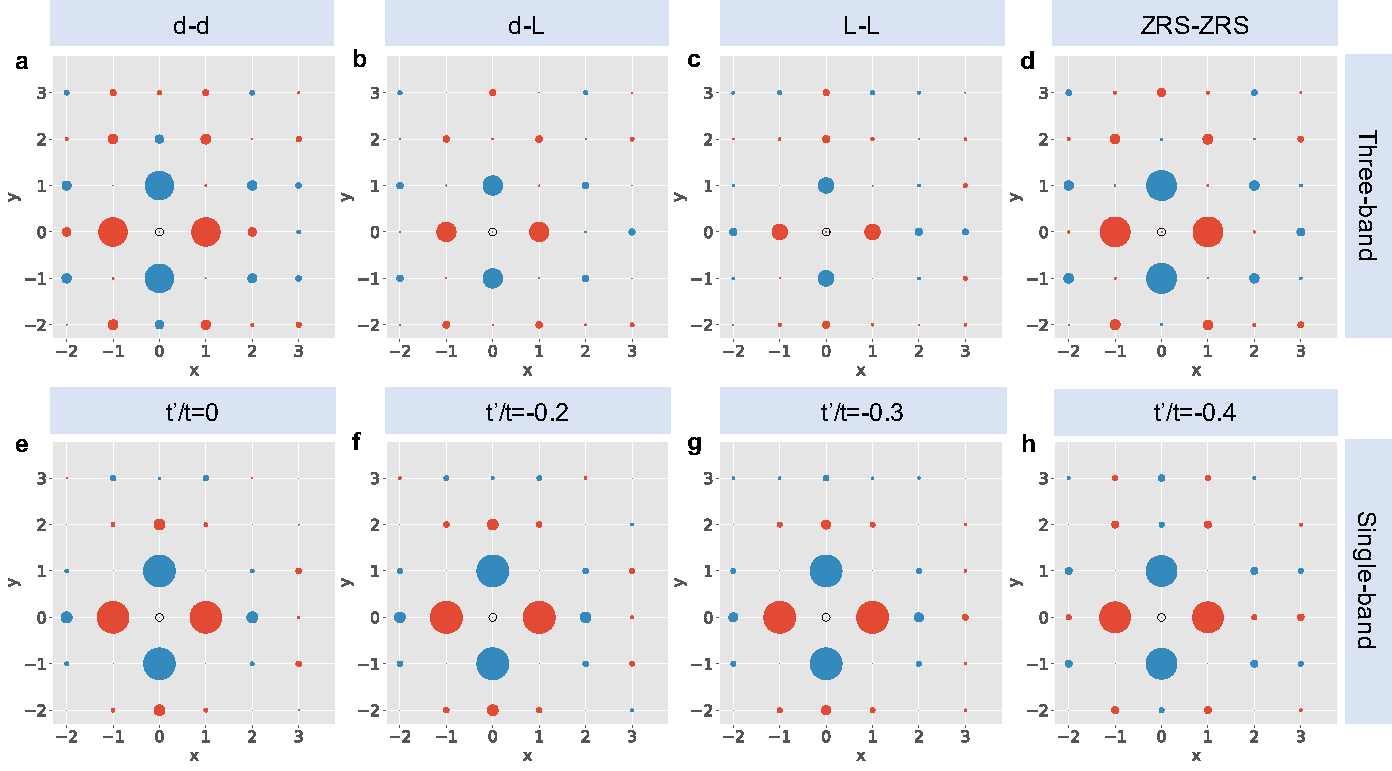
\includegraphics[width=\linewidth]{./Figures/Figure3.pdf}
\caption{{\bf A comparison of the pairing structure in the three-band and single-band models.} Each panel plots the real space components of the leading  particle-particle  BSE  (symmetrized) eigenvector at 15\% hole-doping. The first row shows $d$-$d$, $d$-$L$, $L$-$L$ and ZRS-ZRS pairing components for the three-band model at $\beta=10$ ~eV$^{-1}$. The second row shows the pair structure for the single-band model ($U=6t$, $\beta =5t^{-1}$) at $t^\prime/t=0$,$-0.2$,$-0.3$ and $-0.4$.}
\label{Fig:tbvssb}
\end{figure*}

The orbital structure of the leading eigenvector simplifies considerably after one transforms to the bonding $L$ and anti-bonding $L^\prime$ combinations. Fig.~\ref{Fig:tbvssb} plots the pairing amplitudes for a hole on Cu paired with another hole on a neighboring Cu ($d$-$d$, Fig.~\ref{Fig:tbvssb}{\bf a}) or bonding molecular orbital ($d$-$L$, Fig.~\ref{Fig:tbvssb}{\bf b}). Both components exhibit a clear $d_{x^2-y^2}$ symmetry that is dominated by the (nearest-neighbor) $\cos(k_xa)-\cos(k_ya)$ harmonic; however, both channels also have indications of additional higher order harmonics [i.e. $\cos(2k_xa)-\cos(2k_ya)$ and $\cos(2k_xa)\cos(k_ya)-\cos(2k_ya)\cos(k_xa)$]. Interestingly, the contribution from holes occupying neighboring bonding molecular orbitals exhibits similar behavior ($L$-$L$, Fig.~\ref{Fig:tbvssb}{\bf c}). The $L^\prime$-related pairing contributes very little as will be discussed in Fig.~\ref{Fig:weightvsdensity} and in the supplement (see Supplementary Figure 5)~\cite{supplement}. 

Figs.~\ref{Fig:tbvssb}{\bf a}-{\bf c} establish that the pairing between the different orbital components of the ZRS all possess the requisite $d_{x^2-y^2}$ symmetry. This observation indicates that the ZRS picture  -- a singlet state made up of holes in the $d$ and $L$ orbitals -- is valid for describing pairing correlations in the three-band Hubbard model of the cuprates. To show the pair structure for the ZRS, we plot in Fig.~\ref{Fig:tbvssb}{\bf d} the sum over the $d-d$, $d-L$, $L-d$ and $L-L$ components (with a factor of $0.5$). One sees that the ZRS pair structure has a vanishing $\cos(2k_xa)-\cos(2k_ya)$ component, while higher order harmonics remain. 

To compare with this, we also computed the real-space structure of the leading particle-particle BSE eigenvector for the single-band Hubbard model. Here, we considered cases with next-nearest-neighbor hopping $t^\prime/t = 0$ (panel {\bf e}), $-0.2$ ({\bf f}), $-0.3$ ({\bf g}), which are commonly used in the literature, as well as $-0.4$ ({\bf h}). The single-band model reproduces the short-range pairing structure of the three-orbital model (panel {\bf d}), regardless of the value of $t^\prime$; however, the longer-ranged pairing in Fig.~\ref{Fig:tbvssb}{\bf d} is only captured correctly for large $\big|t^\prime/t \big|$. In particular, we observe that with increasing $\big|t'/t \big|$, the relative amplitude of the third nearest neighbor $[\cos(2k_xa)-\cos(2k_ya)]$ term is suppressed. For $t^\prime/t=-0.4$ (panel {\bf h}), the single-band pair structure is very similar to that for the ZRS (panel {\bf d}), with differences appearing at the longest length scales. This value of $t^\prime$ is close to the value $t^\prime=-0.453t$ that we obtain by downfolding our three-band model parameters onto the single-band model by diagonalizing small Cu$_2$O$_7$ clusters~\cite{Johnston2010,Eskes1991}. A sizeable negative $t^\prime$ is also consistent with parametrizations of the bandstructure extracted from angle-resolved photoemission spectroscopy\cite{ARPES}.  These results provide remarkable support for the validity of the ZRS construction but also indicate that single-band models may not capture the correct longer-ranged correlations without a suitable choice of $t^\prime$. The latter conclusion further underscores the crucial role of $t^\prime$ for determining the superconducting properties of the single-band model~\cite{Maier16, Macridin, Qin2019, Jiang2019}.

\begin{figure}[ht]
\centering
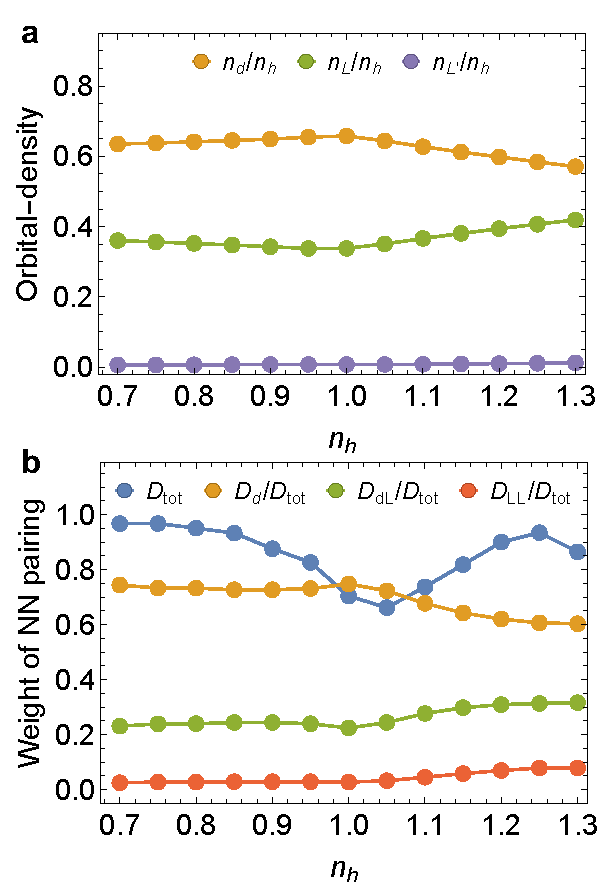
\includegraphics[width=\linewidth]{./Figures/Figure4.pdf}
\caption{{\bf Molecular Orbital compositions in the three-band model.} {\bf a} Ratios of the orbital hole densities to the total density $n_h$. {\bf b} Weights of different orbital compositions of the nearest-neighbor pairs, as defined in Fig.\ref{Fig:PairStructure}, and their total weight. All results were obtained on a $4\times4$ cluster at $\beta=16$~eV$^{-1}$. 
}
\label{Fig:weightvsdensity}
\end{figure}

\subsection*{Weight for different types of pairing}
Figure~\ref{Fig:tbvssb} shows that the structure of the leading eigenvector $\phi_{\alpha\beta}$ is closely linked to the orbital structure of the ZRS. Fig.~\ref{Fig:weightvsdensity} examines how this internal structure evolves with doping by plotting the orbital-dependent hole density (panel {\bf a}) and the orbital composition of the eigenvector $\phi_{\alpha\beta}$ (panel {\bf b}) on a $4\times 4$ cluster (adequate to capture the essential pairing structure) at a lower temperature.  Fig.~\ref{Fig:weightvsdensity}{\bf a} shows that the single hole per unit cell in the undoped case has approximately 65\% Cu-$d$ character, while 35\% of the hole is located in the bonding O-$L$ molecular orbital. With electron doping, there is a small decrease of $n_d/n_h$ indicating that the holes are removed mainly from the Cu-$d$ orbital. In contrast, with hole doping, there is a significant redistribution of the hole density from the $d$- to the $L$-orbital, showing that doped holes mainly occupy the O-$L$ molecular orbital. The hole density on the anti-bonding O-$L^\prime$ orbital is negligible. 

Figure ~\ref{Fig:weightvsdensity}{\bf b} shows that the total weight of the nearest-neighbor pairing increases from $\sim 70$\% in the undoped case to almost 100\% with either hole or electron doping. Since the BSE eigenvector reflects the momentum structure of the pairing interaction, this dependence can be understood from an interaction that becomes more peaked in momentum space as $n_h=1$ is approached. This behavior leads to a more delocalized structure of $\phi_{{\bf r}_\beta}({\bf r}_\alpha)$ and, therefore, a reduction of the relative weight of the nearest-neighbor contribution. The partial contributions to the nearest-neighbor pairing weight, $D_{d}$ and $D_{dL}$, have a doping dependence very similar to the corresponding orbital densities $n_d$ and $n_L$ in panel {\bf a}, closely linking the orbital structure of the pairing to the orbital makeup of the ZRS. The weight of the $L^\prime$ contributions remains negligible over the full doping range~\cite{supplement}. 

\section*{Conclusion}
We have determined the orbital structure of the effective pairing interaction in a three-band CuO$_2$ Hubbard model and shown that it simplifies considerably when viewed in terms of a basis consisting of a central Cu-$d$ orbital and a bonding $L$ combination of the four surrounding O-$p$ orbitals. These states underlie the ZRS singlet construction that enables the reduction of the three-band to an effective single-band model. By explicitly comparing the three-band with single-band results, we showed that the effective interaction is correctly described in the single-band model. In summary, these results strongly support the conclusion that a single-band Hubbard model provides an adequate framework to understand high-$T_c$ superconductivity in the cuprates.

\section*{Methods}
\subsection*{Model parameters}
The three-band Hubbard model we study can be found in Refs.~[\onlinecite{Kung,supplement}]. We adopted a parameter set appropriate for the cuprates~\cite{Kung,Czyzyk,Johnston,Ohta} (in units of eV): the nearest neighbor Cu-O and O-O hopping integrals $t_{pd} = 1.13$, $t_{pp} = 0.49$, on-site interactions $U_{dd} = 8.5$, $U_{pp} = 0$, and charge-transfer energy $\Delta = \varepsilon_p -\varepsilon_d = 3.24$, unless otherwise stated. Since we use a hole language, half-filling is defined as hole density $n_h=1$ and $n_h>1~(<1)$ corresponds to hole (electron)-doping. A finite $U_{pp}$ only leads to small quantitative changes in the results (see Supplementary Fig.~4~\cite{supplement}) but worsens the sign problem significantly~\cite{Kung}. Therefore, we keep $U_{pp}=0$ for this study.

\subsection*{Dynamical cluster approximation}
We study the single- and three-band Hubbard models using DCA with a continuous time QMC impurity solver~\cite{Jarrell,Maier1,Urs,Gull2,Gull3}. 
We determine the structure of the pairing interaction by solving the Bethe-Salpeter equation (BSE) in the particle-particle singlet channel to obtain its leading eigenvalues and (symmetrized) eigenvectors~\cite{supplement, Maier4PRL}. A transition to the superconducting state occurs when the leading eigenvalue $\lambda(T=T_c) = 1$, and the magnitude of $\lambda <1$ measures the strength of the normal state pairing correlations. The spatial, frequency, and orbital dependence of the corresponding eigenvector, which is the normal state analog of the superconducting gap, reflects the structure of the pairing interaction~\cite{Maier16,Maier4PRL}.

\section*{Data Availability} The data that support the findings of this study can be obtained at  \url{https://github.com/JohnstonResearchGroup/Mai_etal_3bandPairs_2021}.

\section*{Code Availability} The DCA++ code used for this project can be obtained at \url{https://github.com/CompFUSE/DCA}.

\section*{Acknowledgements}
Acknowledgements --- The authors would like to thank L. Chioncel, P. Dee, A. Georges, K. Haule, E. Huang, S. Karakuzu, G. Kotliar, H. Terletska, and D.~J. Scalapino for useful comments. This work was supported by the Scientific Discovery through Advanced Computing (SciDAC) program funded by the U.S. Department of Energy, Office of Science, Advanced Scientific Computing Research and Basic Energy Sciences, Division of Materials Sciences and Engineering. This research  used resources of the Oak Ridge Leadership Computing Facility, which is a DOE Office of Science User Facility supported under Contract DE-AC05-00OR22725. 

\section*{Competing interests}
The authors declare no competing interests. 


\section*{Author Contributions}
P.~M., G.~B., and T.~A.~M. developed the DCA++ code. P.~M. carried out the calculations. P.~M., S.~J., and T.~A.~M analyzed the results and wrote the manuscript. S.~J. and T.~A.~M. supervised the project.


\begin{thebibliography}{99}
\bibitem{EmeryPRL1987}
Emery, V. J. Theory of high-T$_\mathrm{c}$ superconductivity in oxides. 
\textit{Phys. Rev. Lett.} {\bf 58}, 2794 (1987). 

\bibitem{ZhangRice}
Zhang, F. C. \& Rice, T. M. Effective Hamiltonian for the superconducting Cu oxides. \textit{Phys. Rev. B}  {\bf 37}, 3759(R) (1988).

\bibitem{Maier4PRL} Maier, T.~A., Jarrell, M.~S. \& Scalapino, D.~J. Structure of the Pairing Interaction in the Two-Dimensional Hubbard Model. \textit{Phys. Rev. Lett.} {\bf 96}, 047005 (2006).

\bibitem{Maier07} Maier, T.~A., Macridin, A., Jarrell, M.~S. \& Scalapino, D.~J. Systematic analysis of a spin-susceptibility representation of the pairing interaction in the two-dimensional Hubbard model. \textit{Phys. Rev. B} {\bf 76}, 144516 (2007).

\bibitem{Maier08} Maier, T.~A., Poilblanc, D. \& Scalapino, D.~J. Dynamics of the Pairing Interaction in the Hubbard and t-J Models of High-Temperature Superconductors. \textit{Phys. Rev. Lett.} {\bf 100}, 237001 (2008).

\bibitem{Kyung09} Kyung, B., Senechal, D. \& Tremblay, A.~M.~S. Pairing dynamics in strongly correlated superconductivity.
 \textit{Phys. Rev. B} {\bf 80}, 205109 (2009).

\bibitem{Gull14} Gull, E. \& Millis, A.~J.
Pairing glue in the two-dimensional Hubbard model. \textit{Phys. Rev. B} {\bf 90}, 041110(R) (2014).

\bibitem{Maier16} Maier, T.~A., Staar, P., Mishra, V., Chatterjee, U., Campuzano, J.C. \&  Scalapino, D.J., Pairing in a dry Fermi sea. \textit{Nat. Commun.} {\bf 7}, 11875 (2016)

\bibitem{Lau11} Lau, B., Berciu, M. \& Sawatzky, G.~A. 
High-Spin Polaron in Lightly Doped CuO$_2$ Planes.  \textit{Phys. Rev. Lett.}  {\bf 106}, 036401 (2011).

\bibitem{Ebra14} Ebrahimnejad, H., Sawatzky, G.~A. \& Berciu, M. The dynamics of a doped hole in cuprates is not controlled by spin fluctuations. \textit{ Nat. Phys.} {\bf 10}, 951 (2014).

\bibitem{Ebra16} Ebrahimnejad, H., Sawatzky, G.~A. \& Berciu, M. Differences between the insulating limit quasiparticles of one-band and three-band cuprate models.
\textit{ J. Phys.: Condens. Matter} {\bf 28}, 105603 (2016).

\bibitem{Adolphs16} Adolphs, C. P. J., Moser, S., Sawatzky, G.~A. \& Berciu, M. Non-Zhang-Rice Singlet Character of the First Ionization State of T-CuO. \textit{Phys. Rev. Lett.} {\bf 116}, 087002 (2016).

\bibitem{Jiang20} Jiang, M., Moeller, M., Berciu, M., \& Sawatzky, G.~A. Relevance of Cu-3d multiplet structure in models of high-T$_c$ cuprates. \textit{Phys. Rev. B} {\bf 101}, 035151 (2020).

\bibitem{Moeller12} M\"{o}ller, M., Sawatzky, G.~A. \& Berciu, M. Magnon-Mediated Interactions between Fermions Depend Strongly on the Lattice Structure. \textit{Phys. Rev. Lett.} {\bf 108}, 216403 (2012).

\bibitem{Chen13} Chen W. \& Sushkov, O.~P. Implications of resonant inelastic x-ray scattering data for theoretical models of cuprates.
 \textit{Phys. Rev. B} {\bf 88}, 184501 (2013).

\bibitem{Dopf}
Dopf, G., Muramatsu, A. \& Hanke, W. Three-band Hubbard model: A Monte Carlo study.
\textit{Phys. Rev. B}, {\bf 41}, 9264 (1990).

\bibitem{Arrigoni}
Arrigoni, E., Daghofer, M., Aichhorn, M., Hanke, W. 
Phase diagram and single-particle spectrum of CuO$_2$ high-T$_c$ layers: variational 
cluster approach to the three-band Hubbard model. 
\textit{New J. Phys.}, {\bf 11}, 055066 (2009).  

\bibitem{Kung} Kung, Y.~F. \textit{et al.} Characterizing the three-orbital Hubbard model with determinant quantum Monte Carlo. \textit{Phys. Rev. B} {\bf 93}, 155166 (2016).


\bibitem{Thomale} Thomale, R. \& Greiter, M. Numerical analysis of three-band models for CuO planes as candidates for a spontaneous T-violating orbital current phase. \textit{Phys. Rev. B}, {\bf 77}, 094511 (2008).

\bibitem{Weber1} Weber, C., Haule, K. \& Kotliar, G. Strength of correlations in electron- and hole-doped cuprates. \textit{Nat. Phys.} {\bf 6}, 574 (2010).

\bibitem{Weber2} Weber, C., Haule, K. \& Kotliar, G. Apical oxygens and correlation strength in electron- and hole-doped copper oxides. \textit{Phys. Rev. B}, {\bf 82}, 125107 (2010).

\bibitem{Weber3} Weber, C., L\"{a}uchli, A., Mila, F. \& Giamarchi, T. Orbital Currents in Extended Hubbard Models of High-$T_c$ Cuprate Superconductors. \textit{Phys. Rev. Lett.} {\bf 102}, 017005 (2009).

\bibitem{Weber4} Weber, C., Giamarchi, T. \& Varma, C.~M. Phase Diagram of a Three-Orbital Model for High-$T_c$ Cuprate Superconductors. \textit{Phys. Rev. Lett.} {\bf 112}, 117001 (2014).

\bibitem{Acharya} Acharya, S. \textit{et al.} Metal-Insulator Transition in Copper Oxides Induced by Apex Displacements. \textit{Phys. Rev. X} {\bf 8}, 021038 (2018).

\bibitem{Biborski} Biborski, A., Zegrodnik, M. \& Spałek, J. Superconducting properties of the hole-doped three-band $d-p$
 model studied with minimal-size real-space $d$-wave pairing operators. \textit{Phys. Rev. B} {\bf 101}, 214504 (2020).
 
\bibitem{Zegrodnik} Zegrodnik, M., Biborski, A., Fidrysiak, M. \& Spałek, J. Superconductivity in the three-band model of cuprates: Variational wave function study and relation to the single-band case. \textit{Phys. Rev. B} {\bf 101}, 214504 (2020).

\bibitem{Huang} E. W. Huang, C. B. Mendl, S. Liu, S. Johnston, H. C. Jiang, B. Moritz and T. P. Devereaux, \textit{Science} {\bf 358}, 1161-1164 (2017).

\bibitem{Cui} 
Cui, Z.-H., Sun, C., Ray, U., Zheng, B.-X., Sun, Q. \& Chan, G. K.-L.,   
Ground-state phase diagram of the three-band Hubbard model from density matrix embedding theory. 
\textit{Phys. Rev. Research} {\bf 2}, 043259 (2020).

\bibitem{KirtleyReview}
Tsuei, C. C. and Kirtley, J. R. Pairing symmetry in cuprate superconductors. 
\textit{Rev. Mod. Phys.} {\bf 72}, 969 (2000).

\bibitem{Maier3} 
 Maier,  T. A., Jarrell, M., Schulthess, T. C., Kent, P. R. C. \& White, J. B. Systematic Study of d-Wave Superconductivity in the 2D Repulsive Hubbard Model. \textit{Phys. Rev. Lett} {\bf 95}, 237001 (2005).
 
\bibitem{Macridin} Macridin, A.,  Jarrell, M.,  Maier, T. A. \& Sawatzky, G. A., Physics of cuprates with the two-band Hubbard model: The validity of the one-band Hubbard model. \textit{Phys. Rev. B} {\bf 71}, 134527 (2005).  

\bibitem{supplement}
See the online supplementary materials.


\bibitem{Moreo} Moreo A. \&  Dagotto, E. Minimal-size real-space d-wave pairing operator in CuO$_2$ planes. \textit{Phys. Rev. B} {\bf 100}, 214502 (2019).

\bibitem{Johnston2010} Johnston, S., Vernay, F., Moritz, B., Shen, Z.-X., Nagaosa, N.,  Zaanen, J., \& Devereaux, T. P. Systematic study of electron-phonon coupling to oxygen modes across the cuprates.  \textit{Phys. Rev. B} {\bf 82}, 064513 (2010). 

\bibitem{Eskes1991} Eskes, H., \& Sawatzky, G. A. Single-, triple-, or multiple-band Hubbard models. \textit{Phys. Rev. B} {\bf 44}, 9656 (1991).


\bibitem{ARPES} Damascelli, A., Hussain, Z. \& Shen, Z. Angle-resolved photoemission studies of the cuprate superconductors. \textit{Rev. Mod. Phys.} {\bf 75}, 473 (2003).

\bibitem{Jiang2019} Y.-F. Jiang, J. Zaanen, T. P. Devereaux, and H.-C. Jiang Ground state phase diagram of the doped Hubbard model on the four-leg cylinder. \textit{Phys. Rev. Research} {\bf 2}, 033073  (2019). 

\bibitem{Qin2019} Qin M. {\it et al.} Absence of Superconductivity in the Pure Two-Dimensional Hubbard Model. Phys. Rev. X {\bf 10}, 031016 (2020). 


% \bibitem{White1989}
% S. R. White, D. J. Scalapino, R. L. Sugar, E. Y. Loh, J. E. Gubernatis, R. T. Scalettar, Phys. Rev. B {\bf 40}, 506 (1989).

% \bibitem{Dahm2009}
% T. Dahm {\it et al.} Nat. Phys. {\bf 5}, 217--221 (2009). 

% \bibitem{Scalapino2012}
% D. J. Scalapino, Rev. Mod. Phys. {\bf 84}, 1383 (2012). 

% \bibitem{Gull} 
% E. Gull, O. Parcollet and A. J. Millis, Phys. Rev. Lett. {\bf 110}, 216405 (2013).


\bibitem{Ohta} Ohta, Y., Tohyama, T. \& Maekawa, S. Apex oxygen and critical temperature in copper oxide superconductors: Universal correlation with the stability of local singlets. \textit{ Phys. Rev. B} {\bf 43}, 2968 (1991).

\bibitem{Johnston} Johnston, S.,  Vernay, F. \&  Devereaux, T. Impact of an oxygen dopant in Bi$_2$Sr$_2$CaCu$_2$O$_8$. \textit{Eur. phys. Lett.} {\bf 86}, 37007 (2009).

\bibitem{Czyzyk} Czy\.{z}yk M. T. \&  Sawatzky, G. A. Local-density functional and on-site correlations: The electronic structure of La$_2$CuO$_4$ and LaCuO$_3$. \textit{Phys. Rev. B} 49, 14211 (1994).

\bibitem{Jarrell} Jarrell, M., Maier, T. A., Huscroft, C. \& Moukouri, S. Quantum Monte Carlo algorithm for nonlocal corrections to the dynamical mean-field approximation. \textit{Phys. Rev. B} {\bf 64}, 195130 (2001).

\bibitem{Maier1} Maier, T. A., Jarrell, M., Pruschke, T. \&  Hettler, M. Quantum cluster theories. \textit{Rev. Mod. Phys.} {\bf 77}, 1027 (2005).

\bibitem{Urs} H\"{a}hner, U. R., Alvarez G., Maier, T. A., Solcà, R., Staar, R., Summers, M. S., Schulthess, T.C. DCA++: A software framework to solve correlated electron problems with modern quantum cluster methods. \textit{Comput. Phys. Commun.} {\bf 246}, 106709 (2020).

\bibitem{Gull2} Gull, E., Werner, P., Parcollet, O., and Troyer, M. Continuous-time auxiliary-field Monte Carlo for quantum impurity models. \textit{Europhys. Lett.} {\bf 82}, 57003 (2008).

\bibitem{Gull3} Gull, E., Staar, P., Fuchs, S., Nukala, P., Summers, M., Pruschke, T., Schulthess, T. and Maier, T. Submatrix updates for the continuous-time auxiliary-field algorithm. \textit{Phys. Rev. B}, {\bf 83}, 075122 (2011).


\end{thebibliography}

% \section*{Publisher’s note}
% Springer Nature remains neutral with regard to jurisdictional claims in published maps and institutional affiliations.


\end{document}